% Capítulo 6
\chapter{Estudo Experimental}
\label{cap:cap6}

Este capítulo consiste em apresentar o estudo por meio do método experimental, envolve a concepção de contexto do experimento, das configurações e características dos elementos envolvidos, a seleção das variáveis influenciadoras, o controle e a instrumentação do experimento, sua execução, a captura de dados durante experimentação, e por fim, a análise e conclusões obtidas a partir desses resultados. 

O objetivo do experimento é analisar a viabilidade do uso de mecanismos de \textit{throttling} como candidato para aumentar a disponibilidade dos elementos presentes em \textit{IoT} através do ajuste de comportamento por ação de limiares de atuação que consideram seus aspectos energéticos para assim,  prolongar a autonomia energética dos dispositivos. A abordagem é aderente e cobre os elementos presentes na taxonomia proposta no Capítulo \ref{cap:cap4} permitindo comparação e análise entre dispositivos que diferem sobre o fato de terem sua operação ajustada mediante \textit{throttling} ou não. 

\section{Metodologia}

O experimento pretende comparar os efeitos do mecanismo de \textit{throttling} em dispositivos com capacidade de coleta de energia, com foco em examinar a disponibilidade de cada um relacionada aos aspectos energéticos em condições de capacidade e atuação semelhantes.

\begin{figure}[H]
	\centering
	\caption{Etapas do Estudo Experimental.}
	\label{fig:cap6metodologia}
	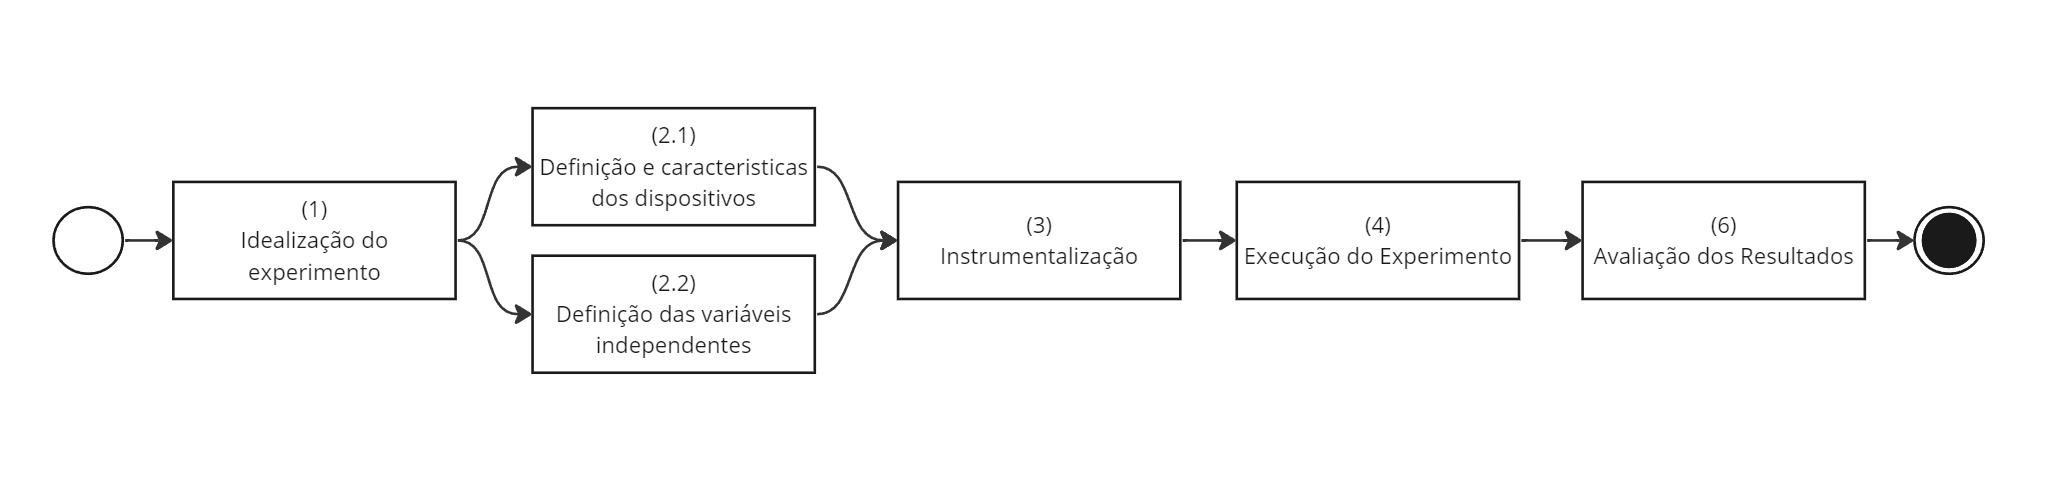
\includegraphics[width=1\linewidth]{Imagens/cap6/cap6metodologia.jpg}
	
	Fonte: elaborado pelo autor.
\end{figure} 

Para tal, buscou-se observar a influência do fator limitante na alteração do comportamento dos participantes em relação aos valores de energia coletada e reserva energética. Além disso, compreender sua eficiência na tomada de decisão em atender ou não às solicitações, em virtude da autoanálise de suas capacidades à medida que a variação de energia disponível ocorre. Este estudo visa analisar o uso de \textit{throttling} como possível solução para estender a disponibilidade de dispositivos com capacidade de coleta energética. 

A Figura \ref{fig:cap6metodologia} apresenta o fluxo de execução e ordem de todas as etapas realizadas. Na Seção \ref{cap6:idealizacao}, foi concebido quais os termos de projeto para viabilizar a análise e comparação de nodes com padrão \textit{throttling} aplicado as características energéticas, este processo caracteriza a Etapa 1. Inicialmente, foi projetado ambiente para abstrair os elementos envolvidos, visando garantir equidade de condições e ações de maneira simultânea para todos os dispositivos durante a simulação. Para alcançar isolamento e consistência, optou-se pelo uso da plataforma Docker\footnote{O Docker é uma plataforma de virtualização que simplifica o desenvolvimento, envio e execução de aplicativos em contêineres. Disponível em \url{https://www.docker.com/}.} como agente facilitador, que atende às restrições necessárias de encapsulamento para que cada aplicação e suas dependências estejam contidas. 

Conforme ilustrado na Figura <DIAGRAMA DE BLOCO DO SISTEMA>, essa abordagem permite que ambos os sistemas fossem estimulados paralelamente, mantendo controle sobre seus recursos e garantindo os termos de operação (capacidade de processador, memória e disco). Sendo assim, a composição do experimento considera que:  I - Dispositivos com capacidade de coleta e armazenamento de energia estão inseridos em um dado ambiente de simulação controlada; II - Os dispositivos sempre recebem simultaneamente o mesmo valor como coleta de energia; III - Os dispositivos participantes possuem a mesma capacidade de armazenamento para energia coletada; IV - Os dispositivos são submetidos simultaneamente a mesma quantidade de solicitações, os ciclos de carga.

Na Etapa 3, abordado-se o processo de instrumentalização do ambiente simulado, essencial meio para apresentar os resultados durante a execução do experimento e posterior resumo dos dados obtidos, seus detalhes estão descritos na Seção \ref{SECAO INSTRUMENTACAO}. A Seção \ref{SECAO EXECUCAO} descreve os processos de execução do experimento Etapa 4, aqui todas as etapas planejadas anteriormente ja estão implementadas. Sendo assim, os procedimentos são realizados conforme o protocolo estabelecido, e aplicação dos estímulos definidos  (carga de solicitações e disponibilização de recursos na forma de coleta energética). Durante esta fase, a precisão e a consistência são fundamentais para garantir a validade dos resultados analisados na próxima fase. 

Ao final, a Etapa 5 trata dos dados coletados para análise e avaliação,
consistindo o grupo de variáveis dependentes: I - Medição dos valores energéticos em relação ao tempo; II - Quantidade de solicitações atendidas ou negadas; III - Valores mínimos de reserva energética atingidos. Tais resultados serão melhores descritos posteriormente e apresentam o escopo de comparação entre os elementos participantes fundamento em que se baseia a avaliação dos resultados descritos na Seção \ref{SECAO AVALIACAO RESULTADOS}.

\section{Idealização}
\label{cap6:idealizacao}
Uma vez definido os objetivos do experimento, a Etapa de idealização é o ponto onde foi construído as bases de execução do estudo. Assim, foram realizadas a estruturação  dos parâmetros e definição do cenário para realizar os testes, além da capacidade de coleta dos resultados e avaliação de conformidade com a taxonomia proposta.

O cenário foi idealizado para simular a atuação dos nodes em dado um ambiente externo. Nele, nodes provedores realizam aferições à medida que são estimulados através de solicitações enviadas. 

Decorrente desta  dinâmica, cabe ao node provedor examinar, com base nas condições energéticas, se é capaz ou não de realizar o comando solicitado. Para tal, o mecanismo de \textit{throttling} deverá atuar observando os recursos energéticos do node provedor, para que ao atingir um determinado limiar, bloquear o atendimento à solicitação realizada.

Ainda nesta etapa, foi necessário considerar as entradas energéticas que seria disponibilizadas ao node provedor, pois devem ser inerentes ao ambiente idealizado onde este node poderia estar inserido. Além disso, concebeu os aspectos de armazenamento dessa entrada energética, dispositivo o qual deverá receber o recurso coletado e disponibiliza-la para uso do node provedor. A Figura \ref{fig:cap6dinamica} ilustra, em resumo, a dinâmica de funcionamento do node.

\begin{figure}[H]
	\centering
	
	\caption{Dinâmica do Node Provedor.}
	\label{fig:cap6dinamica}
	\noindent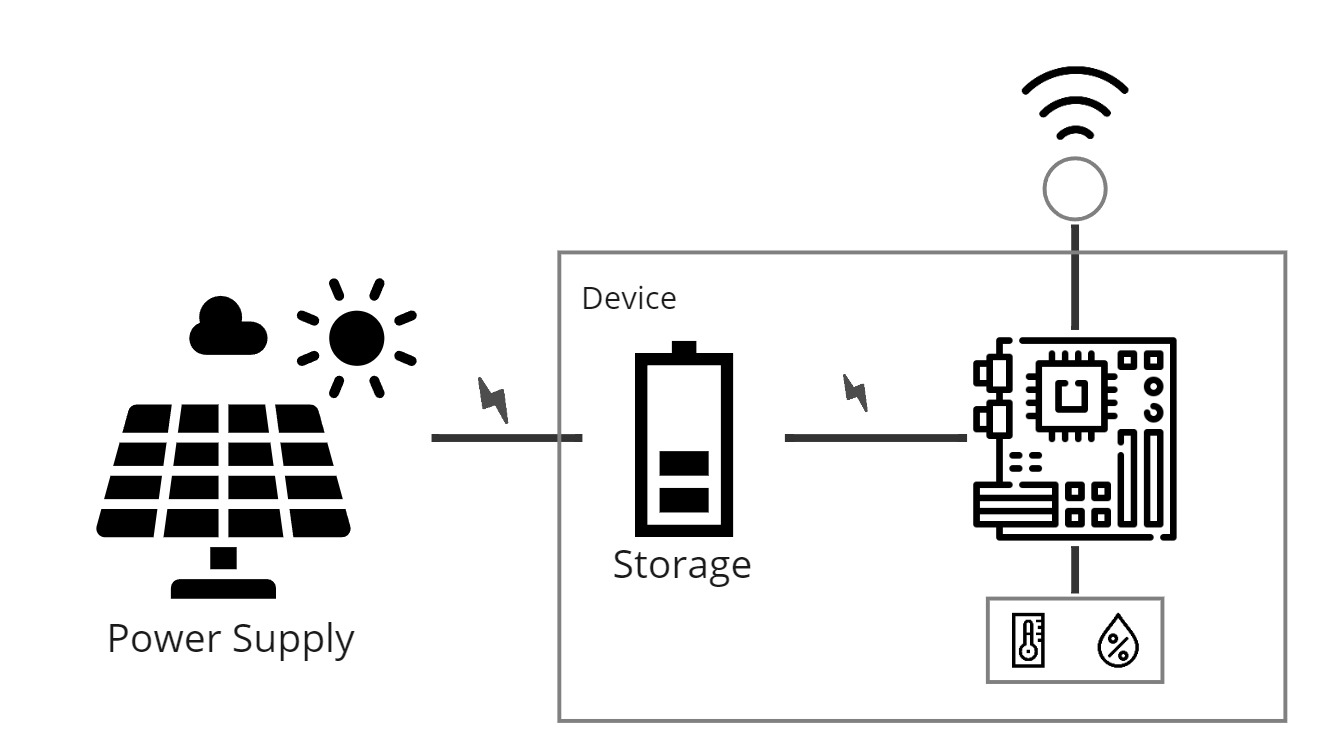
\includegraphics[width=0.75\linewidth]{Imagens/cap6/cap6dinamica.jpg} 
		
	Fonte: elaborado pelo autor.
\end{figure}


Portanto, acontecendo disponibilidade energética, cabe ao dispositivo armazena-la durante um ciclo a medida que os valores vão sendo apresentados ao node. Uma vez cumprido esta etapa, os valores são disponibilizados na forma de recurso que deverá ser dispendido a medida que realiza as atividades solicitadas.

Por fim, o node deverá em todo seu ciclo de vida atuar dinamicamente em conformidade com os modo de operação que represente os valores de recursos energéticos que possui. No experimento estão cobertos quatro modos de atuação a depender das capacidades energéticas:

\begin{enumerate}	
\item Modo Abundante: O Modo Abundante representa o dispositivo que possui recursos energéticos amplamente disponíveis, permitindo o funcionamento completo e otimizado de todas as suas funcionalidades. Aqui, o node atenderá quaisquer solicitação enviada, sem atuação do mecanismo limitante, aproveitando ao máximo a disponibilidade de energia;
\item Modo Atenção: Uma vez atingido este patamar, o node recusar-se a atender algumas solicitações com a motivação de preservar parte dos recursos até que um novo cenário energético seja apresentado;
\item Modo Alerta: O Modo Crítico é alcançado quando o dispositivo está operando com recursos energéticos extremamente limitados, mas ainda tem capacidade para atender algumas solicitações (conforme privilégios ou criticidade das operações). Este modo foi projetado para prolongar a funcionalidade básica do dispositivo enquanto tenta evitar a entrada no Modo Hibernação. 
\item Modo Critico: Este modo é ativado quando o dispositivo não possui mais recursos energéticos suficientes para continuar atendendo qualquer solicitação. O dispositivo entra em um estado de hibernação ou equivalente a um baixo gasto energético para preservar-se até que os recursos energéticos sejam recuperados. Caso consuma toda sua reserva, o dispositivo estará esgotado energeticamente.
\end{enumerate}


Os modos de operação representam o estado energético do node e a atuação do mecanismo de \textit{throttling}, assim evidenciando sua eficiência para o objetivo a medida que pode ou não amortizar o uso energético do node a medida que este reduz a sua capacidade de atendimento as solicitações. Naturalmente, estes modos podem variar, dois modos, tres ou mais podem ser descritos facilmente conforme a especificidade e natureza de cada implementação, sua definição está coberta pelas classes Meios, encontrada na Subseção \ref{cap4:atuacao_meios}.

Estes modos de operação guiam a atuação do mecanismo de \textit{throttling} à medida que baseado nos limiares de atuação, induz uma mudança de estado do nó. A dinâmica dos estados do node pode ser visualizada na Figura \ref{fig:cap6maquinaestados}. De maneira geral, os estados possíveis para o dispositivo são representados como:

\begin{itemize}
	\item Estado Inativo: Aqui o node estará consumindo a menor quantidade de recurso energético possível. Um node inativo se encontra ocioso, sem realizar nenhuma tarefa enquanto aguarda novas solicitações.
	\item Estado Ativo: Um node é considerado ativo enquanto executa solicitações. Nesse estado o node utilizará os recursos energéticos necessários para realização  das atividades mediante o consumo de seus recursos energéticos. 
	\item Estado Desligado: No experimento, o estado desligado é a indicação que o node não tem mais capacidade de assumir qualquer outro estado enquanto não receber recursos energéticos particularmente em decorrência do esgotamento de suas reservas. Portanto, neste estado, um node não realizará qualquer atividade.	
	
\end{itemize}




\begin{figure}[H]
	\centering
	
	\caption{Maquina de estados do Node.}
	\label{fig:cap6maquinaestados}
	\noindent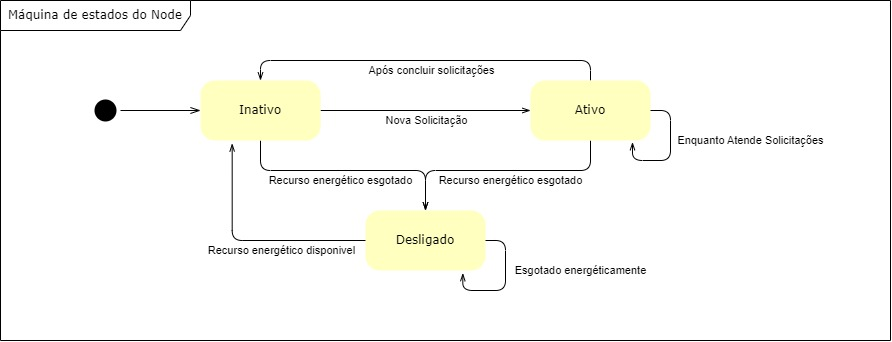
\includegraphics[width=0.75\linewidth]{Imagens/cap6/cap6maquinaestados.jpg} 
	
	Fonte: elaborado pelo autor.
\end{figure}


\section{Definição da variáveis independentes e Dispositivos.}

A teoria de coleta de energia baseia-se na utilização de fontes energéticas disponíveis no ambiente para suprir, parcial ou totalmente, a demanda de um dispositivo. Para o experimento, não há, a princípio, a intenção de analisar cada fonte energética, sua natureza e características particulares de uso ou eficiência energética. 

Com isso, abstraindo sua fonte energética, foi evidenciado para examinação e avaliação da aderência ao mecanismo de \textit{throttling} sob o objetivo proposto, independente da fonte provedora de entrada energética. Quanto a possíveis outras implementações, ainda sim, caberá os ajustes na atuação do \textit{throttling}, neste caso, a depender da especificidade das condições que o node estará submetido, assim como apresentado em \ref{cap:cap4} na classe Observáveis, esses aspectos são descritos como as questões relativas à entrada energética. 

Para execução, compreende a disponibilidade e valores quantitativos da fonte de energia na forma de uma variável independente numérica. Seus valores foram adotados com o auxilio da referencia dos dados disponibilizados no Atlas Brasileiro de Energia Solar \cite{martins2017atlas}. Sendo assim, a definição dos valores de energia disponível orienta-se pelos parâmetros apresentados para cidade de Natal/RN, nos termos da média diária de irradiação solar no decorrer  dos meses. Os valores são expressos em  $Wh/m^2$ , já abstraído a conversão para os termos de consumo conforme Tabela \ref{table:cap6distribuicaonatal}.

\begingroup

\setlength{\tabcolsep}{10pt} % Default value: 6pt
\renewcommand{\arraystretch}{1.5} % Default value: 1

\begin{table}[h]
	
	\centering
	\caption{Média da Disponibilidade Energética Solar Mensal, Natal/RN}
	\smaller[8]
	\tabcolsep=0.1cm
\begin{tabular}{l c | *{13}{c} }
	\toprule
	Momento & $Wh/m^2$ &
	\begin{tabular}{@{}c@{}} 05h00 \\ 0.007\end{tabular} &
	\begin{tabular}{@{}c@{}} 06h00 \\0.02 \end{tabular}	& 
	\begin{tabular}{@{}c@{}} 07h00 \\0.053\end{tabular} &
	\begin{tabular}{@{}c@{}} 08h00 \\0.087 \end{tabular}&
	\begin{tabular}{@{}c@{}} 09h00 \\0.105 \end{tabular}&
	\begin{tabular}{@{}c@{}} 10h00 \\0.127 \end{tabular}& 
	\begin{tabular}{@{}c@{}} 11h00 \\0.136 \end{tabular}& 
	\begin{tabular}{@{}c@{}} 12h00 \\0.125 \end{tabular}& 
	\begin{tabular}{@{}c@{}} 13h00 \\0.12 \end{tabular}& 
	\begin{tabular}{@{}c@{}} 14h00 \\0.101 \end{tabular}& 
	\begin{tabular}{@{}c@{}} 15h00 \\0.074 \end{tabular}& 
	\begin{tabular}{@{}c@{}} 16h00 \\0.04 \end{tabular}&
	\begin{tabular}{@{}c@{}} 17h00 \\0.005 \end{tabular}\\
	
	\hline
	Janeiro & 5674 & 39.72 & 113.48 & 300.72 & 493.64 & 595.77 & 720.6 & 771.66 & 709.25 & 680.88 & 573.07 & 419.88 & 226.96 & 28.37 \\
	\hline
	Fevereiro & 6017 & 42.12 & 120.34 & 318.9 & 523.48 & 631.78 & 764.16 & 818.31 & 752.12 & 722.04 & 607.72 & 445.26 & 240.68 & 30.09\\
	\hline
	Março & 6032 &  42.22 & 120.64 & 319.7 & 524.78 & 633.36 & 766.06 & 820.35 & 754.0 & 723.84 & 609.23 & 446.37 & 241.28 & 30.16\\
	\hline
	Abril & 6082 & 42.57 & 121.64 & 322.35 & 529.13 & 638.61 & 772.41 & 827.15 & 760.25 & 729.84 & 614.28 & 450.07 & 243.28 & 30.41 \\
	\hline
	Maio & 5561 & 38.93 & 111.22 & 294.73 & 483.81 & 583.9 & 706.25 & 756.3 & 695.12 & 667.32 & 561.66 & 411.51 & 222.44 & 27.8 \\
	\hline
	Junho & 5075 & 35.52 & 101.5 & 268.97 & 441.52 & 532.88 & 644.52 & 690.2 & 634.38 & 609.0 & 512.58 & 375.55 & 203.0 & 25.38 \\
	\hline
	Julho & 4658 & 32.61 & 93.16 & 246.87 & 405.25 & 489.09 & 591.57 & 633.49 & 582.25 & 558.96 & 470.46 & 344.69 & 186.32 & 23.29 \\
	\hline
	Agosto & 4773 & 33.41 & 95.46 & 252.97 & 415.25 & 501.16 & 606.17 & 649.13 & 596.62 & 572.76 & 482.07 & 353.2 & 190.92 & 23.87 \\
	\hline
	Setembro & 5571 & 39.0 & 111.42 & 295.26 & 484.68 & 584.95 & 707.52 & 757.66 & 696.38 & 668.52 & 562.67 & 412.25 & 222.84 & 27.86 \\
	\hline
	Outubro & 5971 & 41.8 & 119.42 & 316.46 & 519.48 & 626.95 & 758.32 & 812.06 & 746.38 & 716.52 & 603.07 & 441.85 & 238.84 & 29.86 \\
	\hline
	Novembro & 6112 & 42.78 & 122.24 & 323.94 & 531.74 & 641.76 & 776.22 & 831.23 & 764.0 & 733.44 & 617.31 & 452.29 & 244.48 & 30.56 \\
	\hline
	Dezembro & 6269 & 43.88 & 125.38 & 332.26 & 545.4 & 658.25 & 796.16 & 852.58 & 783.62 & 752.28 & 633.17 & 463.91 & 250.76 & 31.35 \\
\bottomrule
\end{tabular}
\label{table:cap6distribuicaonatal}
\\
\footnotesize Fonte: adaptado de \citeauthor{martins2017atlas}, (\citeyear{martins2017atlas})

\end{table}
\endgroup

A variável independente que representa a entrada energética é provida pela distribuição dos valores médios encontrados em decorrência dos pesos atribuídos para cada ciclo de recarga aqui representado em horas. Os horários suprimidos na Tabela \ref{table:cap6distribuicaonatal} não geram entradas energéticas para o experimento fazendo com que o node receba zero como valor de entrada.

O fator de distribuição atribuído a cada horário representa uma referencia ao impacto da incidência solar naquele momento em relação ao total capturado num intervalo de 24 horas. Para sua realização, foi utilizada a referencia disponibilizada em \citeonline{tutiempo2023} para o dia 12 de dezembro de 2023. A limitação de adotar a distribuição solar para um dia especifico é justificada, pois sua intenção é apenas conceber uma forma para como os dados distribuídos, aproximados das características reais de uma fonte energética solar. Os valores são utilizados como estimulo ao node no decorrer do tempo, e de modo geral, é garantido que, independentemente da distribuição, o montante energético total será disponibilizado integralmente para o node conforme recebe estas entradas. qCom isso, dado o montante energético esperando para um momento, o node receberá seus valores aplicados aos fatores de incidência indicados na  \ref{table:cap6distribuicaonatal} distribuídos em 24 blocos que representam as horas de um dia (00h00 até 23h00).



\subsection{Dispositivos}

Para cobrir a dinâmica idealizada ao node provedor, foi construído os elementos que representam o dispositivo com a capacidade de atuação e os mecanismos do \textit{throttling} inserido em um cenário de restrição energética, uma visão geral do componente pode ser visto na Figura \ref{fig:cap6providernode}. Todo código fonte está disponível no repositório Git para análise e colaboração.\footnote{Código-Fonte do Node Provedor em \url{https://github.com/eusoupaulolopes/mst_experiments}.} 

\begin{figure}[H]
	\centering
	
	\caption{Componentes do Node Provedor.}
	\label{fig:cap6providernode}
	\noindent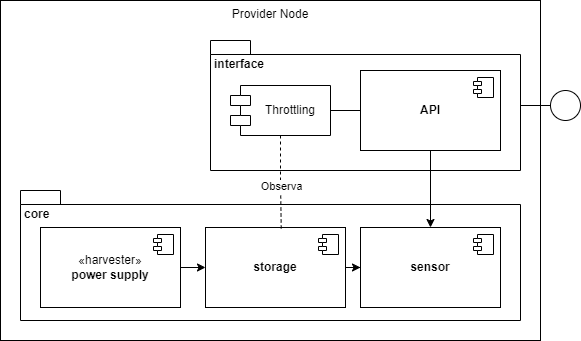
\includegraphics[width=0.75\linewidth]{Imagens/cap6/cap6providernode.png} 
	
	Fonte: elaborado pelo autor.
\end{figure}

\textbf{\\ power supply \\
storage \\
sensor \\ 
interface.}




\section{Instrumentalização.}
\section{Execução.}
\section{Avaliação.}
 